% !TeX program = xelatex
\documentclass{article}
\usepackage{graphicx}
\usepackage{booktabs}
\usepackage{amsmath}
\usepackage{geometry}
\usepackage{float}
\geometry{a4paper,scale=0.8}
\usepackage{listings}
\usepackage{color}
\definecolor{dkgreen}{rgb}{0,0.6,0}
\definecolor{gray}{rgb}{0.5,0.5,0.5}
\definecolor{mauve}{rgb}{0.58,0,0.82}
\lstset{frame=tb,
  language=Python,
  aboveskip=3mm,
  belowskip=3mm,
  showstringspaces=false,
  columns=flexible,
  basicstyle={\small\ttfamily},
  numbers=left,
  numberstyle=\tiny\color{gray},
  keywordstyle=\color{blue},
  commentstyle=\color{dkgreen},
  stringstyle=\color{mauve},
  breaklines=true,
  breakatwhitespace=true,
  tabsize=3
}
\title{实验四\hspace{2em}实验报告}
\author{人工智能2402\hspace{1em}陈子硕}
\usepackage[slantfont,boldfont]{xeCJK}
\usepackage{fontspec}
\usepackage{subcaption}
\usepackage{setspace}
\onehalfspacing
\date{\today}

\begin{document}

\maketitle

\section{实验环境说明}
本次实验在课程服务器上完成，重点考察 PyTorch Distributed Data Parallel（DDP）的基本使用流程，以及 GPU 数量、batch size、模型规模等因素对训练性能和通信开销的影响。

\begin{table}[htbp]
  \centering
  \caption{实验硬件环境}
  \label{tab:hardware_env_exp4}
  \begin{tabular}{p{0.30\linewidth} p{0.62\linewidth}}
    \toprule
    项目 & 配置 \\
    \midrule
    CPU & Intel(R) Xeon(R) Gold 6226R CPU @ 2.90GHz \\
    CPU 拓扑 & 双路，16 cores/socket，2 threads/core，共 64 逻辑 CPU \\
    GPU & NVIDIA GeForce RTX 3090 $\times 8$ \\
    单卡显存 & 24576 MiB（24 GiB） \\
    NVIDIA Driver & 570.133.20 \\
    CUDA（nvidia-smi） & 12.8 \\
    \bottomrule
  \end{tabular}
\end{table}

\begin{table}[htbp]
  \centering
  \caption{实验软件环境}
  \label{tab:software_env_exp4}
  \begin{tabular}{p{0.30\linewidth} p{0.62\linewidth}}
    \toprule
    项目 & 配置 \\
    \midrule
    操作系统 & Linux \\
    Python & Conda 环境 \texttt{ai\_lab} \\
    深度学习框架 & PyTorch（含 \texttt{torch.distributed}） \\
    视觉库 & torchvision \\
    分布式训练方式 & PyTorch DDP \\
    通信后端 & NCCL \\
    \bottomrule
  \end{tabular}
\end{table}

\section{任务一：分布式训练基础实现}
\subsection{实验目标}
本部分的目标是基于 PyTorch 将单机单 GPU 训练改造为分布式数据并行训练，理解 \texttt{rank}、\texttt{local\_rank}、\texttt{world\_size}、\texttt{DistributedSampler} 和 \texttt{DistributedDataParallel} 的作用，并验证程序在多 GPU 环境下能够正常执行。

\subsection{关键实现}
本实验使用 CIFAR-10 数据集，模型选用 ResNet18 与 ResNet50。训练脚本的主要流程包括：
\begin{enumerate}
  \item 使用 \texttt{torch.distributed.init\_process\_group(backend="nccl")} 初始化进程组；
  \item 使用 \texttt{LOCAL\_RANK} 绑定当前进程所使用的 GPU；
  \item 使用 \texttt{DistributedSampler} 对训练集和测试集进行划分；
  \item 使用 \texttt{DistributedDataParallel} 包装模型；
  \item 在训练过程中统计每轮训练耗时、吞吐率和测试准确率；
  \item 通过普通反向传播与 \texttt{model.no\_sync()} 两种方式估算通信开销占比。
\end{enumerate}

核心代码如下：
\begin{lstlisting}[language=Python,caption={实验四训练脚本核心流程},label={lst:ddp_core}]
def setup():
    local_rank = int(os.environ["LOCAL_RANK"])
    world_size = int(os.environ["WORLD_SIZE"])
    rank = int(os.environ["RANK"])
    torch.cuda.set_device(local_rank)
    dist.init_process_group(backend="nccl")
    return rank, local_rank, world_size

train_sampler = DistributedSampler(trainset)
model = build_model(params["model_name"]).to(device)
model = DDP(model, device_ids=[local_rank])
\end{lstlisting}

\subsection{实现说明}
在正式实验前，代码已经能够在 1 卡、2 卡、4 卡和 6 卡条件下稳定运行，终端中能够输出 \texttt{rank=0, local\_rank=0, world\_size=n} 等信息，说明 DDP 的基本链路已经打通。为了减少单次通信测量的随机波动，后续又将每个 epoch 的通信时间测量方式改成了“采样多个 batch 后取平均”。

\begin{figure}[H]
  \centering
  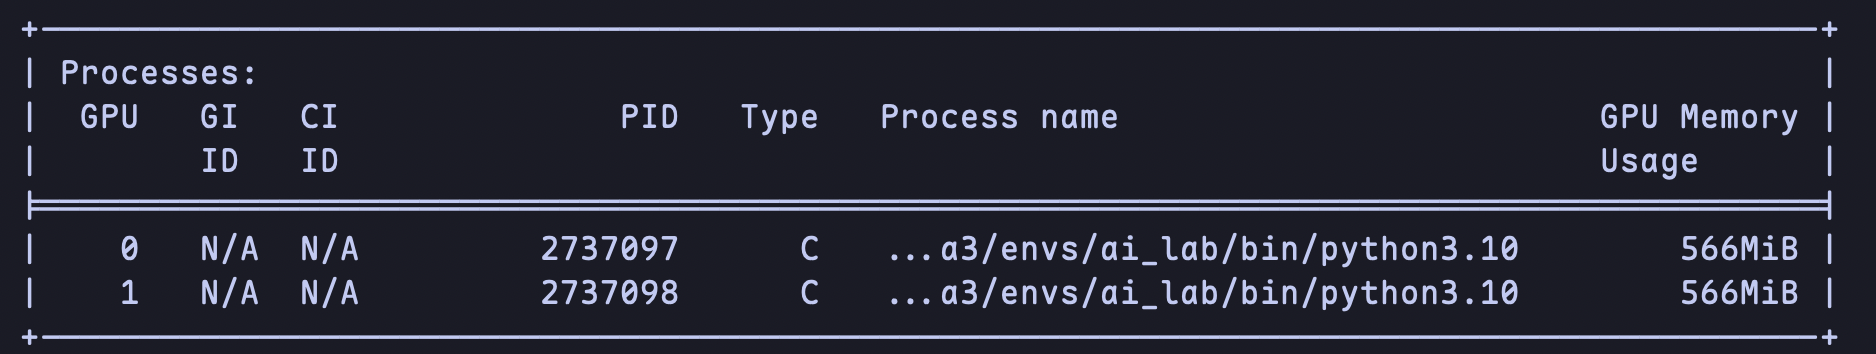
\includegraphics[width=0.95\linewidth]{截屏2026-04-23 11.29.40.png}
  \caption{2 卡 DDP 训练进程运行状态}
  \label{fig:ddp_two_processes}
\end{figure}

\section{任务二：GPU 数量对训练性能的影响}
\subsection{实验设置}
本部分固定模型为 ResNet50，训练 5 个 epoch，每个进程的 batch size 设为 128，分别在 1 卡、2 卡、4 卡和 6 卡条件下运行。记录的指标包括单轮训练耗时、吞吐率、总训练时间以及加速比。

\begin{figure}[H]
  \centering
  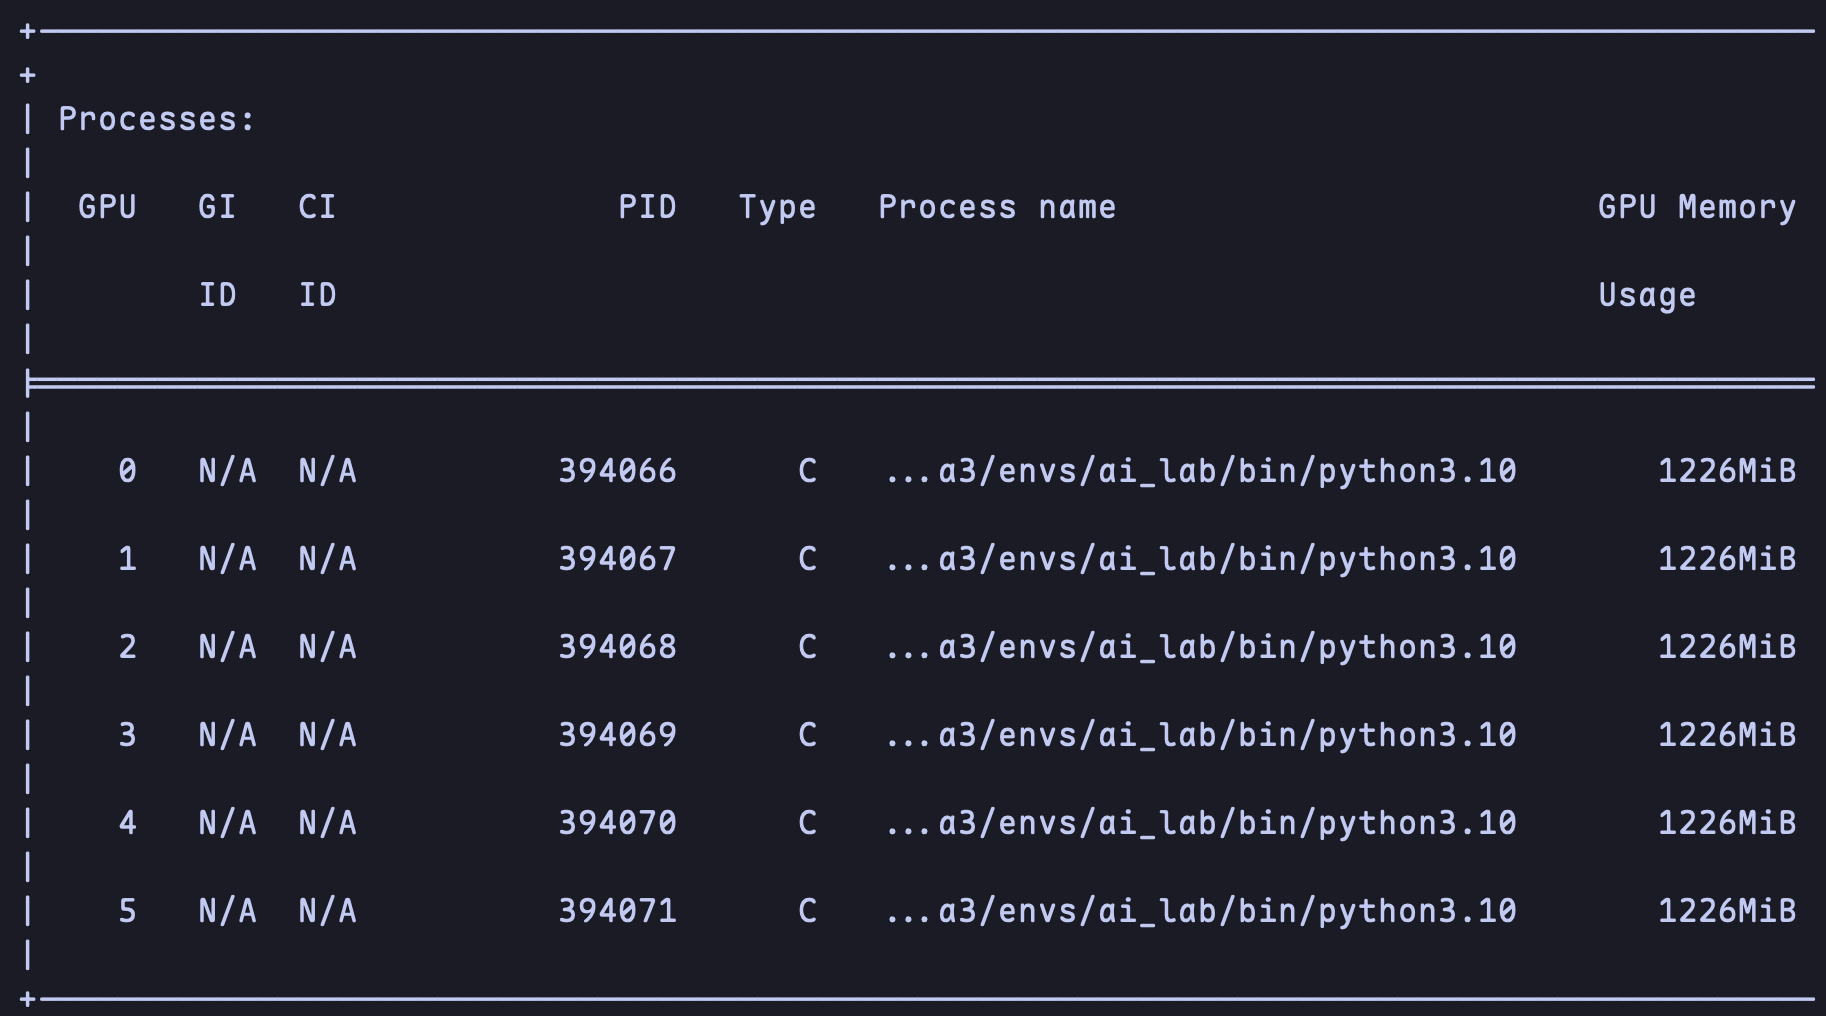
\includegraphics[width=0.95\linewidth]{截屏2026-04-29 10.57.00.png}
  \caption{6 卡 DDP 训练进程运行状态}
  \label{fig:ddp_six_processes}
\end{figure}

\subsection{实验结果}
\begin{table}[H]
  \centering
  \caption{不同 GPU 数量下的训练性能对比}
  \label{tab:gpu_scale_result}
  \begin{tabular}{cccccc}
    \toprule
    GPU 数量 & 总训练时间 / s & 稳定吞吐率 / samples/s & 加速比 & 理想加速比 & 并行效率 \\
    \midrule
    1 & 102.2838 & 约 2790 & 1.00 & 1.00 & 100.0\% \\
    2 & 55.6765 & 约 5330 & 1.84 & 2.00 & 91.8\% \\
    4 & 37.4257 & 约 8145 & 2.73 & 4.00 & 68.3\% \\
    6 & 26.9158 & 约 11805 & 3.80 & 6.00 & 63.3\% \\
    \bottomrule
  \end{tabular}
\end{table}

其中加速比计算方式为：
\[
  \text{Speedup} = \frac{\text{单卡总训练时间}}{\text{当前 GPU 数量下的总训练时间}}
\]

因此：
\[
  \text{2 卡加速比} = \frac{102.2838}{55.6765} \approx 1.84,\quad
  \text{4 卡加速比} = \frac{102.2838}{37.4257} \approx 2.73,\quad
  \text{6 卡加速比} = \frac{102.2838}{26.9158} \approx 3.80
\]

\subsection{结果分析}
从实验结果可以看出，随着 GPU 数量增加，单轮训练耗时明显下降，吞吐率明显上升。1 卡时稳定吞吐率约为 2790 samples/s，2 卡提升到约 5330 samples/s，4 卡进一步提升到约 8145 samples/s，6 卡则提升到约 11805 samples/s，说明 DDP 在单机多卡场景下确实能够带来较明显的训练加速。

但是，加速比并没有达到理想的线性增长。2 卡时加速比为 1.84，并行效率仍然较高；4 卡时加速比为 2.73，并行效率下降到 68.3\%；6 卡时加速比进一步提高到 3.80，但并行效率继续下降到 63.3\%。造成这种现象的主要原因是：GPU 数量增多后，虽然每张卡的计算任务减少，但在反向传播阶段仍然需要进行梯度同步，通信和同步开销变得更加明显，从而限制了扩展效率。

从通信开销占比看，2 卡训练的后 4 轮平均通信占比约为 19.61\%，4 卡约为 57.12\%，6 卡进一步上升到约 57.78\%。这说明当 GPU 数量继续增加时，每张 GPU 上的计算量被进一步分摊，但梯度同步需求并不会相应消失，因此通信和同步开销会在总时间中占据更高比例。

此外，本实验中每个进程上的 batch size 固定为 128，因此 GPU 数量增加时，全局 batch size 也会同步增大。全局 batch size 的变化会影响模型收敛情况，所以不同 GPU 数量下的准确率不适合作为主要对比指标，本任务的重点应放在训练时间、吞吐率和加速比上。

\section{任务三：Batch Size 对通信开销的影响}
\subsection{实验设置}
本部分固定 GPU 数量为 2，模型固定为 ResNet50，训练 5 个 epoch，分别测试 \texttt{batch\_size=64, 128, 256} 三组参数。实验中通过“正常反向传播时间减去 \texttt{no\_sync} 条件下纯计算时间”的方式近似估算通信时间，并以此计算通信开销占比。

\subsection{实验结果}
\begin{table}[H]
  \centering
  \caption{不同 Batch Size 下的通信开销与训练性能}
  \label{tab:batch_size_result}
  \begin{tabular}{ccccc}
    \toprule
    Batch Size & GPU 数量 & 总训练时间 / s & 稳定吞吐率 / samples/s & 后 4 轮平均通信占比 \\
    \midrule
    64 & 2 & 107.3541 & 约 2550 & 17.59\% \\
    128 & 2 & 55.6765 & 约 5300 & 19.61\% \\
    256 & 2 & 47.6404 & 约 6200 & 27.45\% \\
    \bottomrule
  \end{tabular}
\end{table}

后 4 轮平均通信占比的计算如下：
\begin{align*}
  \text{BS=64}:&\ \frac{14.18 + 22.31 + 25.33 + 8.52}{4} = 17.59\% \\
  \text{BS=128}:&\ \frac{19.08 + 19.08 + 19.88 + 20.41}{4} = 19.61\% \\
  \text{BS=256}:&\ \frac{23.01 + 28.24 + 30.83 + 27.73}{4} = 27.45\%
\end{align*}

\subsection{结果分析}
从训练时间和吞吐率看，batch size 增大后，训练吞吐率明显提高，总训练时间整体下降。具体来说，batch size 从 64 增加到 128 再增加到 256 时，稳定吞吐率大致从 2550 samples/s 提升到 5300 samples/s，再提升到 6200 samples/s，说明更大的 batch size 能使 GPU 获得更高的计算利用率。

从通信开销占比看，本次实验结果并没有完全呈现出“batch size 增大，通信占比下降”的理想趋势，反而表现为 64、128、256 三组的平均通信占比依次为 17.59\%、19.61\% 和 27.45\%。这一结果说明本实验中的通信测量仍然存在一定波动。原因在于这里的通信时间是通过近似方法估算得到的，而在实际训练过程中，计算和通信可能存在重叠；同时，CUDA 预热、缓存状态、数据加载和系统调度等因素也会影响单次测量结果。

因此，本任务更稳妥的结论是：增大 batch size 可以稳定提升吞吐率，但通信占比的变化趋势在本次实验中并不完全理想，说明近似测量方法本身存在噪声。报告中应强调这一点，而不是将通信占比结果解释得过于绝对。

\section{任务四：模型参数规模对通信开销的影响}
\subsection{实验设置}
本部分固定 GPU 数量为 2，每个进程的 batch size 固定为 128，训练 5 个 epoch，对比 ResNet18 和 ResNet50 两种不同规模的模型。重点记录模型参数量、总训练时间、吞吐率以及通信开销占比。

\subsection{实验结果}
\begin{table}[H]
  \centering
  \caption{不同模型规模下的训练性能与通信开销}
  \label{tab:model_scale_result}
  \begin{tabular}{lcccccc}
    \toprule
    模型 & 参数量 & GPU 数量 & Batch Size & 总训练时间 / s & 稳定吞吐率 / samples/s & 后 4 轮平均通信占比 \\
    \midrule
    ResNet18 & 11181642 & 2 & 128 & 31.6951 & 约 10200 & 12.96\% \\
    ResNet50 & 23528522 & 2 & 128 & 55.6765 & 约 5300 & 19.61\% \\
    \bottomrule
  \end{tabular}
\end{table}

后 4 轮平均通信占比计算如下：
\begin{align*}
  \text{ResNet18}:&\ \frac{10.82 + 14.72 + 13.18 + 13.12}{4} = 12.96\% \\
  \text{ResNet50}:&\ \frac{19.08 + 19.08 + 19.88 + 20.41}{4} = 19.61\%
\end{align*}

\subsection{结果分析}
从参数规模看，ResNet18 大约有 1118 万个参数，而 ResNet50 大约有 2353 万个参数，后者参数量约为前者的 2.1 倍。从训练性能看，ResNet18 的总训练时间更短，吞吐率明显更高；ResNet50 的训练时间更长，吞吐率更低，这说明模型规模增大后，计算开销也随之增大。

从通信开销占比看，ResNet18 的后 4 轮平均通信占比约为 12.96\%，ResNet50 约为 19.61\%。这一结果更符合直觉：模型参数量越大，在反向传播阶段需要同步的梯度数据也越多，因此通信开销占比更高。

需要说明的是，在本次实验中 ResNet18 的测试准确率高于 ResNet50，但这并不能直接说明 ResNet18 的模型能力一定更强。主要原因是本实验只训练了 5 个 epoch，并且两个模型使用的是同一套超参数设置。对于 CIFAR-10 这种小尺寸图像数据集来说，较浅模型可能更容易在短训练周期内得到较高的准确率。因此，本任务的重点依然是性能和通信开销分析，而不是模型精度对比本身。

\section{任务五：不同通信后端对训练性能的影响（选做）}
\subsection{实验设置}
本部分固定模型为 ResNet50，GPU 数量为 2，每个进程的 batch size 为 128，训练 5 个 epoch，只改变通信后端，对比 NCCL 与 Gloo 在多 GPU 训练下的性能差异。

\subsection{实验结果}
\begin{table}[H]
  \centering
  \caption{不同通信后端下的训练性能与通信开销对比}
  \label{tab:backend_result}
  \begin{tabular}{lcccccc}
    \toprule
    后端 & GPU 数量 & 模型 & Batch Size & 总训练时间 / s & 稳定吞吐率 / samples/s & 后 4 轮平均通信占比 \\
    \midrule
    NCCL & 2 & ResNet50 & 128 & 55.6765 & 约 5330 & 19.61\% \\
    Gloo & 2 & ResNet50 & 128 & 110.1818 & 约 2525 & 57.25\% \\
    \bottomrule
  \end{tabular}
\end{table}

后 4 轮平均通信占比的计算如下：
\begin{align*}
  \text{NCCL}:&\ \frac{19.08 + 19.08 + 19.88 + 20.41}{4} = 19.61\% \\
  \text{Gloo}:&\ \frac{54.19 + 57.70 + 57.47 + 59.64}{4} = 57.25\%
\end{align*}

\subsection{结果分析}
从总训练时间和吞吐率看，NCCL 明显优于 Gloo。在相同实验设置下，NCCL 的总训练时间为 55.6765s，而 Gloo 为 110.1818s，几乎增加到 2 倍；稳定吞吐率方面，NCCL 约为 5330 samples/s，而 Gloo 只有约 2525 samples/s。

从通信开销占比看，NCCL 的后 4 轮平均通信占比约为 19.61\%，而 Gloo 达到 57.25\%，差异非常明显。这说明在 GPU 多卡训练场景下，NCCL 对 GPU 间通信做了更有针对性的优化，而 Gloo 更适合 CPU 或通用分布式通信场景，在 GPU 训练下性能明显较弱。

从准确率看，两种后端在 5 个 epoch 后的最佳准确率接近，NCCL 为 38.95\%，Gloo 为 38.01\%。这说明通信后端主要影响的是训练效率和通信开销，而不会显著改变模型的优化目标本身。

\section{实验中的问题与修复}
实验过程中遇到的主要问题如下：
\begin{itemize}
  \item \textbf{NCCL barrier 警告}：最初直接调用 \texttt{dist.barrier()} 时，终端会出现“devices used by this process are currently unknown”的警告。后续改为 \texttt{dist.barrier(device\_ids=[local\_rank])} 后，该问题得到解决；
  \item \textbf{通信时间波动较大}：一开始每个 epoch 只测量一个 batch 的通信时间，导致 \texttt{Comm Ratio} 波动明显。后续改为采样多个 batch 取平均，结果稳定性有所提升；
  \item \textbf{CPU / DataLoader 影响}：原始脚本中 \texttt{OMP\_NUM\_THREADS} 和 \texttt{num\_workers} 设置偏小，可能影响数据加载效率。后续提高了线程数并将 \texttt{num\_workers} 增加到 4，使测量结果更稳定；
  \item \textbf{单卡通信占比解释问题}：在 \texttt{world\_size=1} 时不存在真正的跨卡梯度同步，因此单卡下的通信占比更多体现为测量噪声和框架额外开销，不能像多卡实验那样直接解释。
\end{itemize}

\section{实验总结}
本次实验围绕 PyTorch DDP 展开，完成了分布式训练基础实现，并进一步从 GPU 数量、batch size 和模型规模三个维度分析了分布式训练性能。结合实验结果，可以得到以下几点结论：
\begin{enumerate}
  \item DDP 能够较方便地将单机单卡训练改造为单机多卡训练，核心步骤包括初始化进程组、配置 \texttt{DistributedSampler} 以及使用 \texttt{DistributedDataParallel} 包装模型；
  \item 随着 GPU 数量增加，吞吐率明显提高、训练时间明显下降，但加速比不会完全线性增长。GPU 数量越多，梯度同步带来的通信和同步开销越明显，最终导致并行效率下降；
  \item 增大 batch size 能稳定提高吞吐率，但本实验中的通信占比没有完全呈现理论上“随 batch size 增大而下降”的趋势，说明近似测量方法本身存在波动和局限；
  \item 模型参数规模增大后，训练时间明显增加，吞吐率下降，同时通信占比也有所上升，这说明在更大规模模型训练中，梯度同步的通信成本会成为重要瓶颈；
  \item 本实验中的通信时间是通过“总时间减去 \texttt{no\_sync} 条件下纯计算时间”近似估算得到的，因此结果应理解为趋势分析而非绝对精确测量。
\end{enumerate}

此外，本次还补做了 NCCL 与 Gloo 的后端对比实验。结果表明，在 GPU 多卡训练场景下，NCCL 的吞吐率明显高于 Gloo，通信开销也显著更低，因此实际工程中应优先选择 NCCL 作为 GPU 分布式训练的通信后端。

除了本次实验内容外，指导书中还提到了多机分布式训练等进一步扩展任务。通过本实验可以看出：在更大规模的大模型训练中，仅靠传统 DDP 往往不够，还需要引入更高效的分布式训练系统，例如 FSDP、DeepSpeed 等，以进一步降低显存压力并优化通信效率。

\end{document}
